\documentclass[12pt, twoside]{article}
\usepackage[letterpaper, margin=1in, headsep=0.5in]{geometry}
\usepackage[english]{babel}
\usepackage[utf8]{inputenc}
\usepackage{amsmath}
\usepackage{amsfonts}
\usepackage{amssymb}
\usepackage{tikz}
\usetikzlibrary{quotes, angles}
\usepackage{graphicx}
\usepackage{enumitem}
\usepackage{multicol}

\newif\ifmeta
\metatrue %print standards and topics tags

\title{Regents Geometry}
\author{Chris Huson}
\date{September 2020}

\usepackage{fancyhdr}
\pagestyle{fancy}
\fancyhf{}
\renewcommand{\headrulewidth}{0pt} % disable the underline of the header
\raggedbottom


\fancyhead[LE]{\thepage}
\fancyhead[RO]{\thepage \\ Name: \hspace{4cm} \,\\}
\fancyhead[LO]{BECA / Dr. Huson / Geometry 08-Area+volume\\* pset ID: 138}

\begin{document}

\subsubsection*{8-6DN-Cross-sections}
\begin{enumerate}
\item %June 2019
    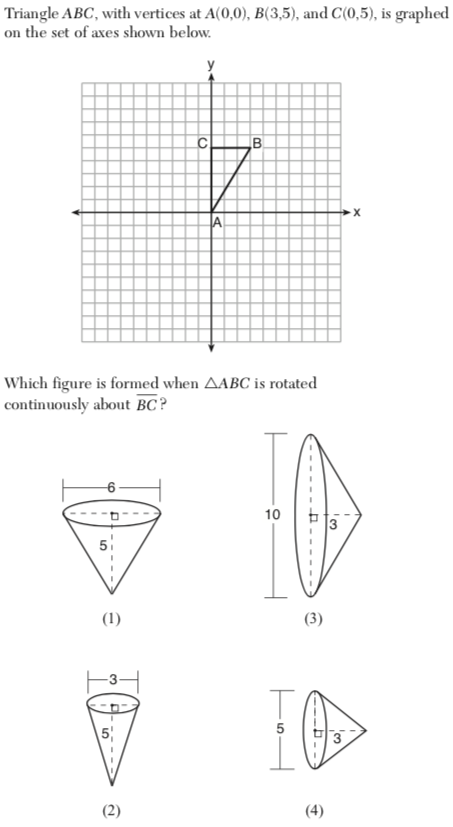
\includegraphics[scale=0.75]{triangle_3d_rotation_JN2018.png}

\newpage
\item %January 2018
  Circle $O$ is centered at the origin. In the diagram below, a quarter of circle $O$ is graphed.
    \begin{center}
      \begin{tikzpicture}[scale=0.6]
        %\draw [help lines] (-4,-4) grid (4,4);
        \draw [thick, <->] (-4,0) -- (4,0) node [below right] {$x$};
        \draw [thick, <->] (0,-3)--(0,3) node [left] {$y$};
        %\draw (0,0) circle [radius=2];
        \draw [thick] (-2,0) arc (180:270:2);
        \node at (0,0) [above right]{$O$};
      \end{tikzpicture}
      \end{center}
    Which three-dimensional figure is generated when the quarter circle is continuously rotated about the $y$-axis?
    \begin{multicols}{2}
      \begin{enumerate}
      \item cone
      \item sphere
      \item cylinder
      \item hemisphere
      \end{enumerate}
    \end{multicols}

\item A student has a rectangular postcard that he folds in half lengthwise. Next, he rotates it continuously about the folded edge. Which three dimensional object below is generated by this rotation?
    \begin{multicols}{2}
    \begin{enumerate}
      \item cone
      \item pyramid
      \item cylinder
      \item rectangular prism
    \end{enumerate}
    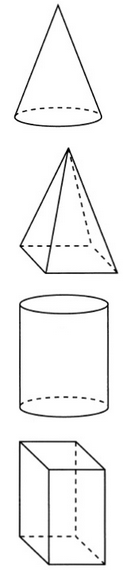
\includegraphics[scale=0.5]{solids.png}
    \end{multicols}

\newpage
\item %June 2019
   If a rectangle is continuously rotated around one of its sides, what is the three-dimensional figure formed?
   \begin{multicols}{2}
    \begin{enumerate}
      \item cone
      \item sphere
      \item cylinder
      \item rectangular prism
    \end{enumerate}
  \end{multicols}

\item %January 2019
  Which three-dimensional figure will result when a rectangle 6 inches long and 5 inches wide is continuously rotated about the longer side?
    \begin{enumerate}
      \item a rectangular prism with a length of 6 inches, width of 6 inches, and height of 5 inches
      \item a rectangular prism with a length of 6 inches, width of 5 inches, and height of 5 inches
      \item a cylinder with a radius of 5 inches and a height of 6 inches
      \item a cylinder with a radius of 6 inches and a height of 5 inches
    \end{enumerate}

\item %August 2018
  An isosceles right triangle whose legs measure 6 is continuously rotated about one of its legs to form a three-dimensional object. The three-dimensional object is a
    \begin{enumerate}
      \item cylinder with a diameter of 6
      \item cylinder with a diameter of 12
      \item cone with a diameter of 6
      \item cone with a diameter of 12
    \end{enumerate}

\item If an equilateral triangle is continuously rotated around one of its medians, which 3-dimensional object is generated?
    \begin{enumerate}
      \item cone
      \item sphere
      \item pyramid
      \item prism
    \end{enumerate}

\newpage
  \subsubsection*{Cross sections of solids} %2 problems in 6 exams

\item %January 2018
  A right hexagonal prism is shown below. A two-dimensional cross section that is perpendicular to the base is taken from the prism.
    \begin{center}
    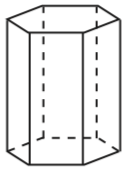
\includegraphics[scale=0.4]{hex-prism_JA2018.png}
    \end{center}
   Which figure describes the two-dimensional cross section?
    \begin{multicols}{2}
      \begin{enumerate}
        \item rectangle
        \item triangle
        \item pentagon
        \item hexagon
      \end{enumerate}
    \end{multicols}

\item  %August 2018
  A right cylinder is cut perpendicular to its base. The shape of the cross section is a
    \begin{multicols}{2}
      \begin{enumerate}
        \item circle
        \item cylinder
        \item rectangle
        \item triangular prism
      \end{enumerate}
    \end{multicols}

\item William is drawing pictures of cross sections of the right circular cone below.
    \begin{center}
      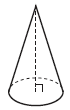
\includegraphics[]{cone.png}
    \end{center}
      Which drawing can \emph{not} be a cross section of a cone?
      \begin{multicols}{2}
      \begin{enumerate}
      \item square
      \item triangle
      \item parabola
      \item ellipse
      \end{enumerate}
      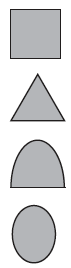
\includegraphics[scale=0.7]{cone-sections.png}
    \end{multicols}

\newpage
\item Which figure can have the same cross section as a sphere?
    \begin{multicols}{2}
      \begin{enumerate}
        \item rectangular prism
        \item pyramid
        \item cone
        \item truncated pyramid
      \end{enumerate}
    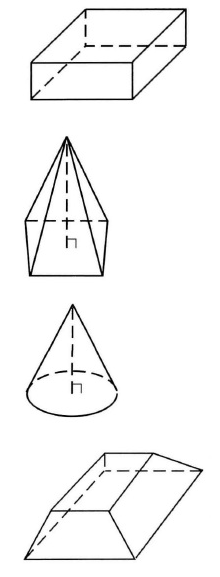
\includegraphics[scale=0.5]{solids2.png}
    \end{multicols}

\item The cross section of a regular pyramid contains the altitude of the pyramid. The shape of this cross section is a
    \begin{multicols}{2}
      \begin{enumerate}
        \item circle
        \item square
        \item triangle
        \item rectangle
      \end{enumerate}
    \end{multicols}

\item A two-dimensional cross section is taken of a three-dimensional object. If this cross section is a triangle, what can not be the three-dimensional object?
    \begin{multicols}{2}
      \begin{enumerate}
        \item cylinder
        \item pyramid
        \item cone
        \item rectangular prism
      \end{enumerate}
    \end{multicols}

\item A plane intersects a hexagonal prism. The plane is perpendicular to the base of the prism. Which two-dimensional figure is the cross section of the plane intersecting the prism?
    \begin{multicols}{2}
      \begin{enumerate}
      \item rectangle
      \item triangle
      \item trapezoid
      \item hexagon
      \end{enumerate}
    \end{multicols}

\end{enumerate}
\end{document}